\chapter[Modelos basados en partes ]{Modelos para detección de objetos basados en partes }\label{ch:capitulo4}
En este capítulo se presenta un análisis en profundidad al framework creado por Felzenszwalb et al. Y el grupo de desarrollo de D. Ramanan, el objetivo principal de este capítulo es presentar y analizar las partes que componen este framework, con el fin de entender su funcionamiento, explorar sus ventajas y analizar las desventajas de éste, tanto para generar los modelos, como para consumirlos en aplicaciones más ligeras. El uso de este framework, básicamente se debe a que nos proporciona un ambiente de desarrollo, el que nos simplifica la realización de muchas tareas. Cabe destacar que este framework fue creado en \textit{MATLAB}, lo que nos permite generar modelos con estructuras ligeras y que pueden ser utilizados por otros lenguajes de programación. En secciones posteriores discutiremos las principales características de este framework, con el objetivo de obtener ventajas significativas para nuestro desarrollo.

\section{Marco de desarrollo}\label{sec:framework}
Para realizar el procesamiento del conjunto de datos se utiliza un framework el cual nos provee de un ambiente acorde a las necesidades de nuestro proyecto, el que nos permitirá generar los modelos para el reconocimiento de objetos y expresiones faciales, a su vez analizaremos la factibilidad de utilizar dicho ambiente para probar nuestro descriptor. Este framework está basado en la estructura de anotaciones del conjunto de imágenes de la base de imágenes PASCAL~\cite{Everingham2010}. Como se mencionó anteriormente este marco está desarrollado en \textit{MATLAB}, con excepción de algunos archivos que fueron escritos en \textit{C/C++} con el fin de poder hacer más rápido los procesos que tienen mayor complejidad de cómputo. Este framework nos permite generar modelos que luego pueden ser consumidos por distintos lenguajes de programación, convirtiendo a este programa en una herramienta de gran ayuda.

\subsection{Definición de datos}\label{sec:datos}
La definición de los datos es una etapa muy importante en este tipo de estudios, ya que esta etapa selecciona la información disponible para ser utilizada en etapas de entrenamiento y prueba. Esta etapa es la encargada de revisar y seleccionar los datos a ser procesados utilizando diversas especificaciones y formas de representación, para dar mejor uso y obtener mejores resultados con los datos de entrada. El preprocesamiento para el marco de desarrollo presentado en este estudio, se utiliza la base de datos PASCAL~\cite{Everingham2010}, la cual provee un conjunto de imágenes y anotaciones---más adelante explicado.

Se necesita detallar información específica de cada imagen, por lo que es necesario crear un archivo XML, con el mismo nombre de la imagen, que contenga la información necesaria para realizar el procesamiento, esto es llamado, anotación. La anotación específica la clase de la muestra, la ruta del archivo; de dónde se obtuvo la imagen; entre otros atributos necesarios de las imágenes de entrenamiento. Lo más importante de estas anotaciones es que contiene la o las \textbf{regiones} de interés, dependiendo de cuántos objetos contenga la imagen. Una región, está representada por cuatro pixeles, los que a su vez, representan los vértices de una diagonal en un plano cartesiano, dónde su origen se encuentra ubicado en la esquina superior izquierda de la imagen. Es importante mencionar, que tanto el eje $x$ como el eje $y$, son positivos, por lo que cada pixel representa la distancia al origen, la forma de una región de interés se presenta en la Figura~\ref{fig:anota} y su archivo XML que representa esta anotación se presenta en el Código~\ref{AnotacionXml} del Anexo~\ref{ch:capIVA}.

\begin{figure}[tb]
 \centering
  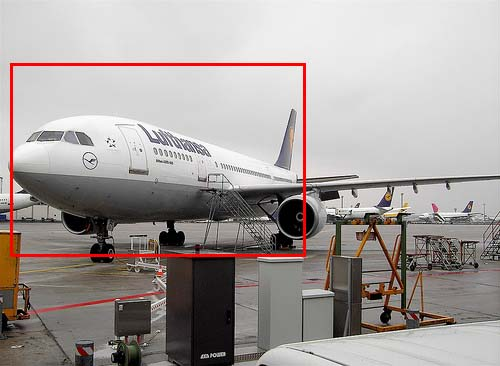
\includegraphics[width=0.8\textwidth]{Figuras/plain.jpg}
  \caption[Región de interés]{Región de interés para un avión. Para un conjunto de imágenes que contienen aviones, las ROI (Regiones de interés), enmarcan las regiones donde se encuentran los objetos pertenecientes a una clase en específico, lo que se utiliza como ejemplo positivo, logrando separar el contenido que no es el objeto en sí mismo, usualmente llamado ejemplos negativos.}
  \label{fig:anota}
\end{figure}

\subsection{Preprocesamiento}\label{subsec:pre}
Una vez creadas todas las anotaciones, se puede iniciar el proceso de creación del modelo. En primera instancia, se agrupan todas las imágenes de acuerdo a la razón entre $w$ (ancho) y $h$ (alto), con lo que se separan los conjuntos de datos en tres partes: datos positivos, es decir, aquellos donde se encuentra el objeto; datos negativos, aquellas imágenes donde no hay presencia de la clase buscada; y finalmente en datos negativos duros, los que contienen imágenes donde hay objetos muy parecidos a simple vista del objeto que estamos buscando clasificar. Finalmente el tamaño de las imágenes será ajustado al promedio de las dimensiones de su razón correspondiente. La estructura del modelo será analizada con mayor detalle en la sección~\ref{sec:model}.

La cantidad de muestras ó tipos de imágenes puede variar influyendo directamente en el resultado, afectando así la efectividad que se haya obtenido en el paso anterior, por lo que es muy importante encontrar y preprocesar un buen conjunto de entrenamiento en una etapa temprana.

\section{Modelo de entrenamiento}\label{sec:model}
Según explica Felzenszwalb et al.~\cite{Felzenszwalb2010}, todos los modelos generados en el framework involucran filtros lineales, los cuales son aplicados a mapas de características densos. De estos mapas se extraen las características más representativas y se crea un vector de características que describe la porción de la imagen que se está observando. A demás, estas características son descritas mediante una variación de HOG el que fue presentado previamente por Dalal and Triggs~\cite{Dalal2005}, aun así este framework es independiente del tipo de extractor de características que se utilice, lo que para nuestro estudio es una ventaja, ya que es aquí donde podemos probar nuestro propio descriptor.

Detalle importante de este framework son los filtros y sus \textit{scores}, ver Sección~\ref{sec:fas}. La idea es definir un \textit{score} que califica en diferentes posiciones y escalas de una imagen el posicionamiento de un filtro, esto es realizado en varios pasos y fases de entrenamiento. Como ejemplo, utilizando imágenes positivas, mediante una pirámide, ver Sección~\ref{sec:pyra}, de características que especifica un mapa de características en un rango fijo, se extraen las características que se extraen por el corrimiento sobre la imagen del filtro raíz, esto se detalla en las siguientes secciones. 

A continuación se presentan las partes más importantes que componen dicho framework, el objetivo es detallar en profundidad el funcionamiento de estos módulos con el fin de adaptar su funcionamiento a nuestro estudio.

\subsection{Deformable Part Models}\label{subsec:dpm}
\textit{Deformable Part Models} son modelos estructurados por un filtro raíz que cubre todo el objeto y por filtros de alta resolución que cubren partes más pequeñas del objeto observado. El filtro raíz define la ventana principal para la detección. Los filtros por cada parte del objeto son ubicados $\lambda$ niveles abajo en la pirámide. Las celdas utilizadas en HOG en cada nivel tienen la mitad del tamaño que las celdas del filtro raíz.
Con estos pasos, Felzenszwalb et al.~\cite{Felzenszwalb2010, Felzenszwalb2013} analizaron que los filtros por partes encuentran características más exactas en resoluciones mayores en comparación con un filtro raíz. Por ejemplo, para un rostro, el filtro raíz podría encontrar los bordes de un rostro y los filtros por partes, los ojos, la boca o la nariz.

Formalmente, un modelo con $n$ partes está definido por un conjunto de parámetros $(F_{0}, (F_{1},d_{1}), \dots, (F_{n}, d_{n}), b)$, donde $F_{0}$ es un filtro raíz, $F_{i}$ es una filtro para una parte del objeto, $d_{i}$ es un vector de parámetros de deformación y $b$ es un escalar. El vector $d_{i}$ especifica los coeficientes de una función cuadrática que especifica el costo de una posible posición para un filtro $i$ relativo a la posición del filtro raíz.

Se genera un hipótesis para un objeto con una vector de configuración $z = (p_{0}, \dots, p_{m})$, donde $p_{i} = (x_{i}, y_{i}, s_{i})$ el que especifica la posición y escala del filtro $i$. El \textit{score} o puntaje de una hipótesis está dado por el \textit{score} de cada parte en su respectiva posición menos un costo de deformación que depende de la posición relativa de cada parte con respecto a la raíz más un escalar de corrección,
\begin{equation}
	\mathit{score}(z) = \sum_{i=0}^n F_{i} \cdot \phi(I, p_{i}) - \sum_{i=1}^{n} d_{i} \cdot \psi(p_{i},p_{0}) + b,
\end{equation}
$$ \text{donde }\psi(p_i. p_0) = (dx_i, dy_i, dx^{2}_i, dy^{2}_i),$$
$$ \text{con } dx_i = x_i-x_0 \text{ y } dy_i = y_i-y_0$$

El \textit{score} de una hipótesis $z$ puede ser expresado en términos de un producto punto, $\beta \cdot \Phi(I, z)$, entre un vector de parámetros de un modelo $\beta$ y un vector de características $\Phi_z$ según propone Felzenszwalb et al.~\cite{Felzenszwalb2013}.

\subsection{Detección}\label{subsec:detection}
Para detectar un objeto en una imagen se calcula un score general sobre la posición del filtro raíz $p_0$ de la imagen de acuerdo al mejor posicionamiento de las partes en relación a $p_0$,
\begin{equation}	\label{max_score}
	\mathit{score}(p_{0}) = \max_{p_{1}, ..., p_{n}} \mathit{score}(p_{0}, ..., p_{n}).
\end{equation}

Una detección está definida por un alto \textit{score} de la posición raíz, mientras que la posición de las partes que cumplen con un \textit{score} alto definen una hipótesis completa de un objeto.

\subsection{Mixture Models}\label{subsec:m_models}
Al existir muchas instancias de una misma clase de objeto, que por ejemplo muestran distintos puntos de vistas, es normal extender la estrategia de tener un modelo por objeto a crear un modelo que mezcle todas esas instancias con el fin de crear un modelo unificado de un objeto, esto recibe el nombre de \textit{Mixture Models}.

Para detectar objetos utilizando \textit{Mixture Models}, primero se calculan los \textit{scores} acumulado de las raíces de forma independiente para cada componente, y luego para cada ubicación del filtro raíz se selecciona la hipótesis del componente de puntuación más alta en ese lugar.

Formalmente, \textit{Mixture Models} está definido como $m$-tuplas, $M = (M_1, \dots, M_m)$, donde $m$ es la cantidad de componentes, es decir $m$ modelos, $M_c$ representa al modelo para el $c$-avo componente. Una hipótesis para un objeto, $z = (c, P_0, \dots, P_{n_c})$ para \textit{Mixture Models} especifica un \textit{Mixture Component}, $1 \leq c \leq m$, y una posición $p_i$ para cada filtro de $M_c$. El \textit{score} o puntaje para esta hipótesis de objeto es el puntaje obtenido por la hipótesis $z^{\prime} = (c, P_0, \dots, P_{n_c})$ para el componente $c$. Al igual que para un modelo simple el \textit{score} de una \textit{Mixture Models} es el producto punto entre el vector de parámetros del modelo y su correspondiente vector de características que depende de la imagen $I$ y una hipótesis $z$.

\section{Latent SVM}\label{sec:lsvmIV}
Los modelos creados por este marco de desarrollo utilizan clasificadores lineales con variables latentes. Para poder entrenar a estos clasificadores se utiliza \textit{Latent} \textit{support} \textit{vector} \textit{machine} (\textit{LSVM}). Para la creación de LSVM se crea la siguiente función:

\begin{equation}\label{lsvm_f}
f_{\beta}(x) = max_{z \in Z(x)} \beta \cdot \Phi (x, z).
\end{equation}
Donde $x$ es una entrada, por ejemplo, una ventana de detección; $\beta$ es un vector con los parámetros del modelo; y $z$ son los valores asignados de las variables latentes de una parte posicionada. El conjunto $Z(x)$ define los posibles valores latentes para una muestra $x$.

Como analogía al tradicional SVM, se puede entrenar $\beta$ desde ejemplos etiquetados de la forma $D = (\langle x_1, y_1 \rangle, \dots, \langle x_n, y_n \rangle)$, donde $y_i \in \{-1, 1\}$, minimizando la siguiente función objetivo:
\begin{equation}\label{o_function}
L_D(\beta) = \frac{1}{2} \Vert \beta \Vert^2 + C \sum_{i=1}^n {\rm max} (0, 1-y_if_\beta (x_i)),
\end{equation}
donde ${\rm max} (0, 1-y_if_\beta(x_i))$ representa la función estándar de pérdida Hinge y la constante $C$ controla el peso relativo del término de regularización. Dado que el valor de la función~\ref{lsvm_f} es no lineal en $\beta$, la función objetivo~\ref{o_function} de LSVM es no convexa en $\beta$. Sin embargo, el problema de entrenamiento se vuelve convexo una vez la información latente es especificada para los ejemplos de entrenamiento positivos.

Felzenszwalb et al.~\cite{Felzenszwalb2010} explica que $f_{\beta}(x)$ como se define en ~\ref{lsvm_f}, es un máximo de la funciones donde cada una es lineal en $\beta$. Por lo tanto, $f_{\beta}(x)$ es convexa en $\beta$. Esto implica que la función de pérdida Hinge es convexa en $\beta$ con $y_i = -1$. Por lo que la función de pérdida es convexa en $\beta$ para ejemplos negativos, esta propiedad es llamada \textit{semi-convexidad}.

Debido a esto la función de pérdida Hinge en LSVM, no es convexa para ejemplos positivos ya que es el máximo de una función convexa (cero) y una función cóncava $(1-y_if_{\beta}(x_i))$.

Esto es muy importante ya que si consideramos un LSVM donde solo hay un solo valor latente posible para cada ejemplo positivo. En ese caso, $f_{\beta}(x)$ es lineal para un ejemplo positivo y la pérdida debido a cada ejemplo positivo es convexa. Combinando esto con la propiedad semi-convexa el resultado se vuelve convexo en $\beta$.

\section{Modelos de entrenamiento}\label{subsec:t_models}

Teniendo un conjunto de imágenes para entrenar, cada una de ellas con sus regiones de interés marcando los objetos de una determinada categoría o clase, por ejemplo, de la clase botella, la región de delimitada será aquella donde se encuentra una botella. Se definen ejemplos positivos por cada una de estas regiones. Estas regiones no especifican etiquetas para los \textit{mixture} \textit{component} o la posición de los filtros, por lo tanto estos son tratados como variables latentes durante el proceso de entrenamiento.
La información que hay dentro de las regiones se usa para poder posicionar el filtro raíz en cada ejemplo positivo. A su vez se define un conjunto de ejemplos negativos grande, donde no hay presencia de los objetos de la categoría que se está analizado.
Por cada posición y escala de una imagen entrega un ejemplo negativo diferente.

El objetivo de separar las imágenes en ejemplos positivos y negativos tiene directa relación con la implementación de LSVM donde la idea principal es obtener un puntaje alto para los ejemplos positivos y un puntaje bajo para los ejemplos negativos, para esto se utiliza el algoritmo presentado en la Sección~\ref{sec:lsvmIV}.

El proceso de entrenamiento consta de varias etapas que a continuación se detallan:

\textbf{Inicialización del filtro raíz}:
Para cada categoría automáticamente se seleccionan las dimensiones del filtro raíz tomando en cuenta el tamaño promedio de las regiones de interés definidas en los datos de entrenamiento. El filtro raíz inicial $F_0$ es entrenado usando SVM normal sin variables latentes. Los ejemplos positivos son extraídos desde el conjunto de ejemplos de entrenamiento sin traslape, es decir donde el objeto es 100\% visible (Estos vienen etiquetados en el conjunto de datos que proporciona PASCAL). Estos ejemplos son reescalados cuidadosamente al tamaño y razón del filtro. Ventanas aleatorias son creadas en las imágenes negativas para generar ejemplos negativos.

\textbf{Actualización del filtro raíz}:
Teniendo en cuenta el filtro raíz inicial formado en el paso anterior, para región delimitante en el conjunto de entrenamiento se encuentra la mejor puntuación de la posición del filtro que se superpone significativamente con la región de interés definida en los datos de entrenamiento. Esto se hace en la imagen original solamente, en las imágenes creadas no. Luego se re-entrena $F_0$ con el nuevo conjunto positivo y los ejemplos negativos aleatorios, haciendo esto dos veces.

\textbf{Inicialización de las partes}:
En esta etapa se inicializa la cantidad de partes, siendo estas declaradas al momento de inicializar el algoritmo de entrenamiento, Felzenszwalb et al.~\cite{Felzenszwalb2008}, inicializa seis partes desde el filtro entrenado en el paso anterior. Primero, se seleccionan una área $a$ tal que $6a$ sea igual al 80\% del área del filtro raíz. Gradualmente se seleccionan regiones rectangulares de la área $a$ del filtro raíz que posee la mayor energía positiva. Los pesos de las regiones se definen en cero y luego se repite el proceso hasta que seis partes son seleccionadas. Los filtros por partes son inicializados con los valores del filtro raíz en la subventana seleccionada por la parte, pero usan relleno para las partes con mayor resolución. Los costos iniciales de la deformación se miden con la norma cuadrada del desplazamiento con $a_i=(0, 0)$ y $b_i=-(1, 1)$.

\textbf{Actualización del modelo}:
Para actualizar el modelo se construyen nuevo datos de entrenamiento, se separan los tres conjuntos de entrenamiento. Para cada región positiva en el conjunto de entrenamiento, se aplica el detector existente en todas las posiciones y escalas con al menos un 50\% de superposición con la región delimitadora dada. Entre esos datos de entrenamiento se seleccionan las posiciones con puntuación más alta en los ejemplos positivos correspondientes a la región delimitada.

Los ejemplos negativos son seleccionados desde las imágenes que no contienen el objeto y entregan un puntuación elevada con la detección. Se añaden los ejemplos negativos a un caché hasta que se llega al límite del tamaño del archivo, esto se declara en un archivo externo de configuración. Un nuevo modelo es entrenado corriendo \textit{SVMLight} en los ejemplos positivos y negativos, cada uno etiquetado con las posiciones de las partes. Se actualiza el modelo 10 veces usando los datos guardados en caché. En cada iteración se guardan los casos difíciles del caché anterior y se añaden tantos nuevos casos complicados como sea posible dentro del límite de la memoria. En las iteraciones finales, podemos incluir todas las instancias de los casos difíciles, en el caché.

\section{Resumen}\label{sec:summaryIV}

Como se pudo ver a través de este capítulo, este framework nos otorga el ambiente de desarrollo propicio para probar nuestra propuesta, ya que al ser un framework modular, nos permite hacer cambios en distintos puntos del framework, logrando así obtener mejoras, he incluso nos permite conocer con mayor detalle el enfoque realizado para su construcción.
El objetivo de este capítulo es presentar las principales partes de este programa, esto nos abre las posibilidades para hacer modificaciones, buscando así optimizar su rendimiento y encaminando su desarrollo para implementar nuestra propuesta y así probar su funcionamiento con nuestra propuesta para objetos y expresiones faciales. Como se verá en los siguientes capítulos el análisis de este framework está directamente relacionado con las futuras pruebas que ser harán para comprobar los resultados obtenidos por nuestro descriptor. Es de suma importancia presentar este framework ya que es este programa el que nos ayudará a probar nuestra propuesta con el fin de poder lograr mejoras interesantes.



